\documentclass[11pt,letterpaper]{article}
\usepackage{epsfig}
\usepackage{graphicx}
\usepackage{graphics}  
\usepackage{cite}      % bibliographic sitations 
\usepackage{floatflt}  
\usepackage{fancybox}  %allows for shadow boxes etc.
\usepackage{color}     %allows use of colors (RBG only, I think)
\usepackage{html}      % allows easy inclusion of links which are
                       % interpretted properly by both latex and latex2html
\topmargin -0.5in
\setlength{\textwidth}{6.5in}
\setlength{\textheight}{8.75in}
\setlength{\oddsidemargin}{0in}
\setlength{\evensidemargin}{0in}

%
%%%%%%%%%%%%%%%%%%%%%%%%%%%%%%%%%%%%%%%%%%%%%%%%%%%%%%%%%%%%%%%%%%%%%
%

\begin{document}

%
%%%%%%%%%%%%%%%%%%%%%%%
% Define new commands %
%%%%%%%%%%%%%%%%%%%%%%%
%
% choose one of the following definitions of mycomment (second = good copy)
\newcommand{\mycomment}[1]{\marginpar{\it\tiny #1}} % used for margin comments
%\newcommand{\mycomment}[1]{\typeout{#1}}
\newcommand{\txt}[1]{{\mbox{\tiny #1}}} %facilitates sub/superscripts
                                        % that aren't italicized
\newcommand{\order}{{\cal O}}

\newenvironment{mylist}
{\begin{list}{}{
  \setlength{\leftmargin}{0.5cm}
  \setlength{\itemsep}{0pt}
  \setlength{\parsep}{0pt}
  \setlength{\topsep}{0pt}
  \renewcommand{\makelabel}{}}}
{\end{list}}

\newenvironment{myitemize}[1]
{ \begin{small}
  \vspace{-.2cm} {\bf \underline{\sc #1}} \vspace{-.2cm}
  \begin{itemize}
  \setlength{\itemsep}{-4pt}
  \setlength{\parsep}{0pt}
  \setlength{\topsep}{0pt}
  \setlength{\partopsep}{0pt}
}
{\end{itemize}\end{small}}
\newcommand{\myitem}[2]{ \item {\bf #1}: {\it #2} }

% from page 4 of fancybox.sty manual
\newenvironment{fminipage}%
{\begin{Sbox}\begin{minipage}}%
{\end{minipage}\end{Sbox}\fbox{\TheSbox}}
%
% use 
% \begin{fminipage}{3in} 
%     the text paragraph is 3 inchs wide
% \end{fminipage}
% to have a multi-line framed box
%
%%%%%%%%%%%%%%%%%%%%%%%%%%%%%%%%%%%%%%%%%%%%%%%%%%%%%%%%%%%%%%%%%%%%%
%
\begin{titlepage}
{\tiny \LaTeX-ed on \today.}

\vspace{2cm}

\begin{center}

{\Huge\bf HepMC 2}

\vspace{1cm}

{\huge a C++ Event Record for Monte Carlo Generators }

\vspace{2cm}

\htmladdnormallink{http://savannah.cern.ch/projects/hepmc/}
{http://savannah.cern.ch/projects/hepmc/}

\vspace{1cm}

{\Large User Manual Version 2.04} \\
May 6, 2008

\vspace{2cm}

{\huge Matt Dobbs} \\
University of Victoria, Canada

\vspace{.2cm}

{\Large J$\o$rgen Beck Hansen} \\
CERN

\vspace{.2cm}

{\Large Lynn Garren} \\
Fermi National Accelerator Laboratory

\vspace{.2cm}

{\Large Lars Sonnenschein} \\
CERN

\vspace{1cm}

\end{center}
\begin{abstract}
  The HepMC package is an object oriented event record written in C++
  for High Energy Physics Monte Carlo Generators.  Many extensions
  from HEPEVT, the Fortran HEP standard, are supported: the number of
  entries is unlimited, spin density matrices can be stored with each
  vertex, flow patterns (such as color) can be stored and traced,
  integers representing random number generator states can be stored,
  and an arbitrary number of event weights can be included.  Particles
  and vertices are kept separate in a graph structure, physically
  similar to a physics event.  The added information supports the
  modularisation of event generators.  The package has been kept as
  simple as possible with minimal internal/external dependencies.
  Event information is accessed by means of iterators supplied with
  the package. 

  HepMC 2 is an extension to the original HepMC written by Matt Dobbs.
\end{abstract}
\end{titlepage}

\setcounter{page}{1}
\tableofcontents

\newpage

%
%%%%%%%%%%%%%%%%%%%%%%%%%%%%%%%%%%%%%%%%%%%%%%%%%%%%%%%%%%%%%%%%%%%%%
%

\section{Introduction}
This user manual is intended as a companion to the 
\htmladdnormallinkfoot{online documentation}
{http://lcgapp.cern.ch/project/simu/HepMC/},
and together with the examples
should provide a friendly introduction to the HepMC event record. A
general overview is available in Ref.~\cite{dobbs:2000CompPhysComm}.

The HEP community has moved towards Object-Oriented computing tools
(usually C++): most upcoming experiments are choosing OO software
architecture, and Pythia 8~\cite{Torbjorn} and 
Herwig++~\cite{Richardson}, written in C++, are available.  
A standard event record must be simple for the end user to access information,
while maintaining the power and flexibility offered by OO design. The
HepMC event record has been developed to satisfy these criteria.

HepMC is an object oriented event record written in C++ for Monte
Carlo Generators in High Energy Physics. It has been developed
independent of a particular experiment or event generator.  It is
intended to serve as both a ``container class'' for storing events after
generation and also as a ``framework'' in which events can be built up
inside a set of generators. This allows for the modularisation of
event generators---wherein different event generators could be
employed for different steps or components of the event generation
process (illustrated in Figure~\ref{modularisation}).
\footnote{
%
At the {\it Physics at TeV Colliders Workshop 2001} in Les
Houches, France, a group of Monte Carlo authors and experimentalists
produced a document~\cite{Boos:2001cv} which outlines the information
content necessary for two event generators to communicate information
about a hard process to the subsequent stages of event
generation. This was implemented in a set of Fortran common blocks,
and many ideas from HepMC were used, such as the scheme for handling
color flow information. Version 1.1 of HepMC supports the full event
information content of Ref.~\cite{Boos:2001cv} (run
information---pertaining to a collection of events---is also specified
in that document and is not addressed in HepMC).  }

\begin{figure}[h]
  \begin{center}
    \Ovalbox{\begin{minipage}{5in}\begin{small}
        \begin{tabular}{rcl}
          $\overbrace{\mbox{Hard~Process~Generator}}^{
            \mbox{\color{magenta}Specific NLO Generator}}$ &
          $\stackrel{\rm \color{blue}Event~Record}{\rightarrow\rightarrow}$ &
          $\overbrace{\mbox{Cascade~Package}}^{
            \mbox{\color{magenta}ARIADNE}}$ \\
          &
          $\stackrel{\rm \color{blue}Event~Record}{\rightarrow\rightarrow}$ &
          $\overbrace{\mbox{Hadronization~Package}}^{
            \mbox{\color{magenta}Herwig}}$ \\
          &
          $\stackrel{\rm \color{blue}Event~Record}{\rightarrow\rightarrow}$ &
          $\overbrace{\mbox{Decay~Package}}^{
            \mbox{\color{magenta}EvtGen}}$ \\
          &
          $\stackrel{\rm \color{blue}Event~Record}{\rightarrow\rightarrow}$ &
          $\overbrace{\mbox{Detector~Simulation}}^{
            \mbox{\color{magenta}ATLfast}}$ \\
        \end{tabular}\end{small}
      \end{minipage}}\end{center}
  \caption{\label{modularisation} 
    HepMC supports the concept of modularised event generation
    (illustrated above) by containing sufficient information within the
    event record to act as a messenger between two modular steps in
    the event generation process.  }
\end{figure}


Physics events are generally visualised using diagrams with a graph structure
(Figure~\ref{graph_structure}, left) which HepMC imitates by separating
out particles from vertices and representing them as the edges and
nodes respectively of a graph~\footnote{
  Ref.~\cite{mc++} uses a similar structure.} 
(Figure~\ref{graph_structure}, right). Each vertex maintains a listing of
its incoming and outgoing particles, while each particle points back
to its production vertex and decay vertex.
The extension to  multiple collisions is natural - the 
super-position of graphs from several different initial processes - 
and so the event may contain an unlimited number 
of (possibly interconnected) graphs. 
The number of vertices/particles in each event is also open-ended.
A subset of the event (such as one connected graph or a single vertex
and its descendants) may be examined or modified without having to
interpret complex parent/child relationship codes or re-shuffle the rest 
of the event record.

\begin{figure}[h]
  \begin{center}
     \parbox[c]{55mm}{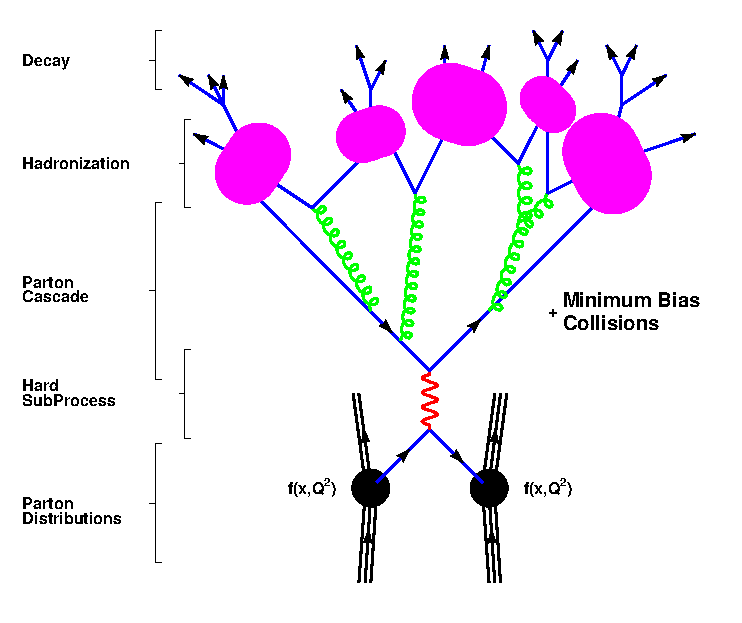
\includegraphics[height=45mm,clip=]
       {physicist_visualization.eps}}
     \mbox{\huge ${\stackrel{\rm HepMC}{\rightarrow}}$}
     \parbox[c]{45mm}{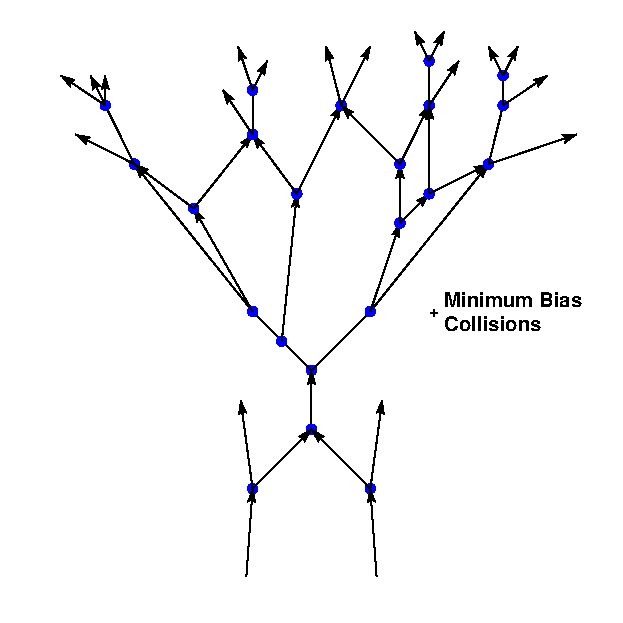
\includegraphics[height=45mm,clip=]
       {graph_interpretation.eps}}
  \end{center}
  \caption{\label{graph_structure} Events in HepMC are stored in a graph
    structure (right), similar to a physicist's visualisation of a
    collision event (left).}
\end{figure}

%
%%%%%%%%%%%%%%%%%%%%%%%%%%%%%%%%%%%%%%%%%%%%%%%%%%%%%%%%%%%%%%%%%%%%%
%

\subsection{Features of the HepMC Event Record}

\begin{itemize}\setlength{\itemsep}{0pt}
\item simple - easy access to information provided by iterators
\item minimum dependencies
\item information is stored in a graph structure, 
  physically similar to a collision event
\item allows for the inclusion of spin density matrices 
\item allows for the tracing of an arbitrary number of flow patterns
\item ability to store the state of random number generators (as
  integers)
\item ability to store an arbitrary number of event weights
\item strategies for conversion to/from HEPEVT (Ref.~\cite{Boos:2001cv}) 
  which are easily extendible to support other event records
\item strategies for input/output to/from ascii files which
  are easily extendible to support other forms of persistency
\end{itemize}

%
%%%%%%%%%%%%%%%%%%%%%%%%%%%%%%%%%%%%%%%%%%%%%%%%%%%%%%%%%%%%%%%%%%%%%
%

\section{HepMC 2}

Since January 2006, HepMC has been supported as an LCG external package.
The official web site is now \htmladdnormallink 
{http://savannah.cern.ch/projects/hepmc/} 
{http://savannah.cern.ch/projects/hepmc/}, 
and compiled libraries for supported platforms are available at 
/afs/cern.ch/sw/lcg/external/HepMC.

Historically, HepMC has used CLHEP (Ref.~\cite{clhep}) Lorentz vectors.  Some users wished to use
a more modern Lorentz vector package.  At the same time, 
there was concern about allowing dependencies on any external package.  
Therefore, the decision was made to replace the CLHEP Lorentz vectors with
a minimal vector representation within HepMC.  

Because this is a major change, the versioning is changed 
from 1.xx.yy to 2.xx.yy.  Normally, a version number change in \emph{xx} 
represents a change to the code and a version number change in \emph{yy}
represents a bug fix.

There have also been continuing requests for other features.
Changes to HepMC must be approved by the LCG simulation project.  

%
%%%%%%%%%%%%%%%%%%%%%%%%%%%%%%%%%%%%%%%%%%%%%%%%%%%%%%%%%%%%%%%%%%%%%
%

\subsection{Overview of Changes Since HepMC 1.26}

See the HepMC ChangeLog~\cite{changelog} for a complete listing.

GenEvent now contains pointers to a heavy ion class and a PDF information class.
The pointers are null by default.  
In addition, GenEvent now has the capability to declare which
momentum and position units are used.

GenParticle momentum and GenVertex position are represented by a simple FourVector 
class instead of the CLHEP Lorentz vectors.  
The SimpleVector.h header contains the FourVector and ThreeVector classes.
GenVertex will return the ThreeVector portion of the position.
Polarization will accept or return a ThreeVector representation 
of the polarization.

Both FourVector and ThreeVector have templated constructors.  
These constructors allow you to use the GenParticle and GenVertex constructors
with \emph{any} Lorentz vector, as long as the Lorentz vector has 
\verb!x()!, \verb!y()!, \verb!z()!, and \verb!t()! methods.

The generated mass, which has always been part of the HEPEVT common block, 
is now stored in GenParticle.  
When a particle has large momentum and small mass, 
calculating the mass from the momentum is unreliable.
Also, different machine representations and roundoff errors mean that
a calculated mass is not always consistent.
If no generated mass is set, then the mass is calculated from the momementum 
and stored in GenParticle.

The IO\_AsciiParticles class provides output in the Pythia style.
This output is intended for ease of reading event output, not for persistency.

The IO\_Ascii output class is deprecated in favor of IO\_GenEvent, 
described in Section~\ref{iogenevent}.  
IO\_GenEvent persists all information in the updated GenEvent object and
uses iostreams for greater flexibility.  IO\_GenEvent also has a 
constructor taking a file name and mode type for backwards compatibility. 
Output remains in ascii format.

%
%%%%%%%%%%%%%%%%%%%%%%%%%%%%%%%%%%%%%%%%%%%%%%%%%%%%%%%%%%%%%%%%%%%%%
%

\section{Package Structure}

Entries within the event record are separated into particles and
vertices. Each particle is composed of momentum, flow, and
polarization classes as well as id and status information. 
The vertices are the connection nodes
between particles and are a container class for particles: thus each
particle within an event belongs to at least one vertex. In addition
the vertex is composed of position, id, and (spin density matrix) 
weight information. Particles and vertices are uniquely identified by
an integer---referred to as a ``barcode''---which is meant to be a
persistent label for a particular particle instance.
The event is the container class for all (possibly
inter-connected) vertices in the event and contains process id, event
number, weight, and random number state information.

Iterators are provided as methods of the vertex and event classes
which allow easy directed access to information in the C++ Standard
Template Library (STL) style.

The event record class relationships and the particle
data class relationships are shown in Figure~\ref{UML_diagrams}.

\begin{figure}[h]
  \begin{center}
    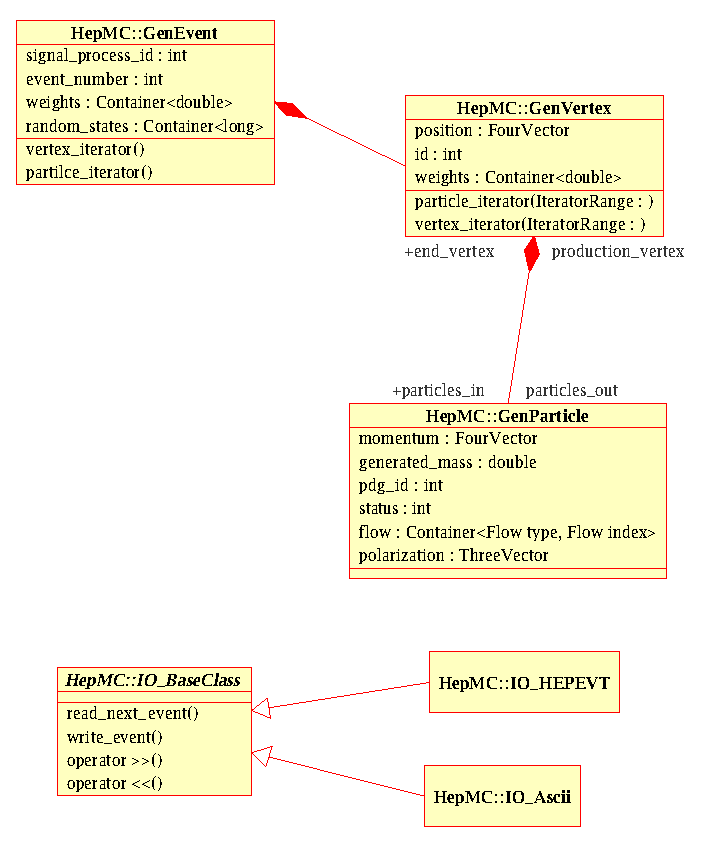
\includegraphics[width=\textwidth,clip=]{HepMC_basic_properties.eps}
  \end{center}
  \caption{\label{UML_diagrams} Class diagrams for the event record
    classes (GenEvent, GenVertex, and GenParticle) and the IO strategies
    are shown in the UML notation.}
\end{figure}

Several input/output strategies are provided. The interface for these
strategies is defined by an abstract base class, IO\_BaseClass.  These
strategies are capable of input/output of events and as such they depend 
directly on the event record class.

The package consists of about 5500~lines of code including
$\approx$1500~comments. There are 7 core classes (GenEvent,
GenVertex, GenParticle, Flow, Polarization, WeightContainer,
IO\_BaseClass) and several utility classes (i.e.\ IO\_HEPEVT, IO\_GenEvent,
HEPEVT\_Wrapper, PythiaWrapper, \ldots).

\subsection{Dependencies}

The HepMC 2 package  depends only on the C++ Standard
Template Library~\cite{stl} (STL).

The HepMC 1 package dependencies were limited to STL 
and the vector classes from the
Class Library for High Energy Physics~\cite{clhep} (CLHEP).  

Simple wrappers for the Fortran versions of Pythia~\cite{Sjostrand:2001yb} 
and Herwig~\cite{herwig} are supplied with the
package to allow the inclusion of event generation examples.

\subsection{Namespace}

The HepMC package is written within the HepMC:: namespace. Outside of
this namespace all class names will need to be prefixed by HepMC::.

\subsection{Performance}

The CPU time performance of the HepMC event record has been quantified
by generating 1000 LHC $W\gamma$ production events using Pythia 5.7
and transferring the event record to HepMC using the IO\_HEPEVT
strategy. Results are summarised in Table~\ref{benchmarks}.
Generation of events in Pythia required 29 seconds of CPU time.
Generating the same events and transferring them into HepMC required
34 seconds.

\begin{table}[h]
\begin{center}
\begin{tabular}{|l l l|c|c|} \hline
&&&CPU Time & File Size \\ \hline
Pythia &           &          & 29 sec & \\
       & + {\color{red}HepMC}   &          & 34 sec & \\ \hline
       & + {\color{red}HepMC} & + {\color{red}IO\_Ascii} 
       & 64 sec & 60.5 Mbytes \\
       & + {\color{green}LCWRITE} &          
       & 92 sec & 106 Mbytes \\
\multicolumn{3}{|l|}{HEPEVT raw size 1K events, 500K particles}
&& 48.2 Mbytes \\ \hline
\end{tabular}
\end{center}
\caption{\label{benchmarks} 
  CPU time performance and file size using a dedicated 450 MHz Pentium~III.}
\end{table}

The time to write HepMC events as ascii files using the IO\_Ascii
strategy was compared to \verb!LCWRITE!, a simple Fortran routine used
in NLC studies to write the HEPEVT common block in formatted ascii to file.
Generating the events with Pythia, transferring them to HepMC, and
writing them to file took 64~seconds and produced a 60.5~Mbyte file.
Generating the events with Pythia and writing them to file using the
\verb!LCWRITE! subroutine took 92~seconds and produced a 106~Mbyte
file. Compression algorithms (such as \verb!gzip!) can reduce the file
sizes by a factor 3 or more.  The raw size of the HEPEVT common block
for these 1000~events (which in this case produced about 500K~particles) is
48.2~Mbytes.  In both cases most CPU time is spent writing to file.
HepMC benefits from added logic when interpreting the record and from 
position information which is stored once for each vertex, rather than
with every particle.  

CPU time savings will be realized when HepMC is
used inside event generators - since it is possible to target and
modify one area of the particle/vertex graph without re-shuffling the
rest of the event record.

%
%%%%%%%%%%%%%%%%%%%%%%%%%%%%%%%%%%%%%%%%%%%%%%%%%%%%%%%%%%%%%%%%%%%%%
%
\section{Overview of Core Classes}

\underline{\bf NOTE ABOUT UNITS}:
HepMC does not define which units are used for the information stored
in the event record.
The HEPEVT standard uses GeV/mm, and so the output from most Fortran
generators will normally be in these units.
CLHEP and Geant4 use MeV/mm, and some collaborations such as ATLAS
have adopted these units for their simulation.

As of HepMC 2.04.00, GenEvent contains member data to store information
about units used.  We recognize that while units may be defined, 
HepMC itself will not know what the units are unless the user specifies them.
Therefore, units are "unknown" until set by the user.
Setting units to UNKNOWN is a choice required for backwards compatibility
with persistent GenEvents created by previous versions of HepMC.
However, we strongly encourage users to declare units 
for {\bf forward} compatiblity.  
It may be that units will be required in some future release.

HepMC users should refer to the code that fills the event record 
to determine which units are being used.

%
%%%%%%%%%%%%%%%%%%%%%%%%%%%%%%%%%%%%%%%%%%%%%%%%%%%%%%%%%%%%%%%%%%%%%
%

\subsection{HepMC::GenEvent}
\begin{myitemize}{Important Public Methods}
  \myitem{add\_vertex}{adopts the specified vertex to the event and
    assumes responsibility for deleting the vertex}
  \myitem{remove\_vertex}{removes the specified vertex from the event,
    the vertex is not deleted - thus use of this method is normally
    followed directly by a delete vertex operation}
  \myitem{vertex\_iterator}{iterates over all vertices in the event -
    described in the iterator section}
  \myitem{particle\_iterator}{iterates over all particles in the event
    - described in the iterator section}
  \myitem{vertex\_const\_iterator}{constant version of the vertex\_iterator}
  \myitem{particle\_const\_iterator}{constant version of 
	the particle\_iterator}
  \myitem{print}{gives a formatted printout of the event to the
    specified output stream}
  \myitem{barcode\_to\_particle}{ returns a pointer to the particle
  	associated with the integer barcode argument }
  \myitem{barcode\_to\_vertex}{ returns a pointer to the vertex
  	associated with the integer barcode argument }
  \myitem{set\_units}{set both momentum and position units}
  \myitem{set\_momentum\_units}{set the momentum units using the momentum enum}
  \myitem{set\_position\_units}{set the position units using the position enum}
  \myitem{convert\_momentum\_units}{convert from, for instance, GeV to MeV}
  \myitem{convert\_position\_units}{convert from, for instance, mm to cm}
\end{myitemize}
\begin{myitemize}{Relevant Data Members}
  \myitem{signal\_process\_id}{an integer ID uniquely specifying the
    signal process (i.e.\ MSUB in Pythia).}
  \myitem{event\_number}{integer}
  \myitem{event\_scale}{(optional) the scale of this event.
	(-1 denotes unspecifed)}
  \myitem{alphaQCD}{(optional) the value of the strong coupling
    constant $\alpha_{QCD}$
	 used for this event. (-1 denotes unspecifed)}
  \myitem{alphaQED}{(optional) the value of the electroweak coupling
    constant $\alpha_{QED}$ (e.g.\ $\frac{1}{128}$)
	 used for this event. (-1 denotes unspecifed)}
  \myitem{signal\_process\_vertex}{(optional) pointer to the vertex
    defined as the signal process - allows fast navigation to the core
    of the event}
  \myitem{beam\_particle\_1}{(optional) pointer to the first incoming beam particle }
  \myitem{beam\_particle\_2}{(optional) pointer to the second incoming beam particle }
  \myitem{weights}{a container of an arbitrary number of 8 byte 
    floating point event weights}
  \myitem{random\_states}{a container of an arbitrary number of 4 byte
    integers which define the random number generator state just
    before the event generation}
  \myitem{heavy\_ion}{(optional) a pointer to a HeavyIon object 
                      (zero by default)}
  \myitem{pdf\_info}{(optional) a pointer to a PdfInfo object 
                     (zero by default)}
  \myitem{momentum\_units}{momentum units (UNKNOWN, MEV, or GEV)}
  \myitem{position\_units}{position units (UNKNOWN, MM, or CM)}
\end{myitemize}
\begin{myitemize}{Notes and Conventions}
  \item if hit and miss Monte Carlo integration is to be performed
    with a single event weight, the first weight will be used by default
  \item Memory allocation: vertex and particle objects will normally
    be created by the user with the NEW operator. Once a vertex
    (particle) is added to a event (vertex), it is "adopted" and
    becomes the responsibility of the event (vertex) to delete that
    vertex (particle).
\end{myitemize}

The GenEvent is the container class for vertices. 
A listing of all vertices is maintained with the event, giving fast
access to vertex information. GenParticles are accessed by means of the
vertices.

Extended event features (weights, random\_states, heavy\_ion, pdf\_info) 
have been implemented such that if left empty/unused performance and memory
usage will be similar to that of an event without these features.

Iterators are provided as members of the GenEvent class
(described in Section~\ref{iterators}). Methods which fill containers of
particles or vertices are {\it not provided}, as the STL provides these
functionalities with algorithms such as \verb!copy! and iterator adaptors
such as \verb!back_inserter! giving a clean generic approach.
Using this functionality it is easy to obtain lists of
particles/vertices given some criteria - such as a list of all final
state particles. Classes which provide the criteria (called
predicates) are also {\it not provided}, as the number of
possibilities is open ended and specific to the application -
and would clutter the HepMC package. Implementing a predicate is
simple (about 4 lines of code).
Examples are given in the GenEvent header file and in
\verb!example_UsingIterators.cc! (Section~\ref{examples}).

The signal\_process\_id is packaged with each event (rather than being
associated with a run class for example) to handle the possibility of
many processes being generated within the same run. A container of
tags specifying the meaning of the weights and random\_states entries
is envisioned as part of a run class - which is beyond the scope of an
event record.

%
%%%%%%%%%%%%%%%%%%%%%%%%%%%%%%%%%%%%%%%%%%%%%%%%%%%%%%%%%%%%%%%%%%%%%
%

\subsubsection{HepMC::PdfInfo}
\begin{myitemize}{Relevant Data Members}
  \myitem{id1}{flavour code of first parton}
  \myitem{id2}{flavour code of second parton }
  \myitem{pdf\_id1}{LHAPDF set id of first parton}
  \myitem{pdf\_id2}{LHAPDF set id of second parton}
  \myitem{x1}{fraction of beam momentum carried by first parton ("beam side")}
  \myitem{x2}{fraction of beam momentum carried by second parton ("target side")}
  \myitem{scalePDF}{Q-scale used in evaluation of PDF's (in GeV)}
  \myitem{pdf1}{PDF (id1, x1, Q)  This should be of the form x*f(x)}
  \myitem{pdf2}{PDF (id2, x2, Q)  This should be of the form x*f(x)}
\end{myitemize}
\begin{myitemize}{Notes and Conventions}
  \item The LHAPDF\cite{lhapdf} set ids are the entries in the first column of
	\htmladdnormallink
	{http://projects.hepforge.org/lhapdf/PDFsets.index}
	{http://projects.hepforge.org/lhapdf/PDFsets.index}.
  \item The LHAPDF set ids pdf\_id1 and pdf\_id2 are zero by default.
  \item IMPORTANT: The contents of pdf1 and pdf2 are expected to be x*f(x), 
        which is the quantity returned by LHAPDF.
  \item IMPORTANT: Input parton flavour codes id1 and id2 are expected to 
        obey the PDG code conventions, especially g = 21. 
\end{myitemize}

PdfInfo stores additional PDF information for a GenEvent.
Creation and use of this information is optional. 

%
%%%%%%%%%%%%%%%%%%%%%%%%%%%%%%%%%%%%%%%%%%%%%%%%%%%%%%%%%%%%%%%%%%%%%
%

\subsubsection{HepMC::HeavyIon}
\begin{myitemize}{Relevant Data Members}
  \myitem{Ncoll\_hard}{Number of hard scatterings}
  \myitem{Npart\_proj}{Number of projectile participants}
  \myitem{Npart\_targ}{Number of target participants}
  \myitem{Ncoll}{Number of NN (nucleon-nucleon) collisions}
  \myitem{N\_Nwounded\_collisions}{Number of N-Nwounded collisions}
  \myitem{Nwounded\_N\_collisions}{Number of Nwounded-N collisons}
  \myitem{Nwounded\_Nwounded\_collisions}{Number of Nwounded-Nwounded collisions}
  \myitem{spectator\_neutrons}{Number of spectators neutrons}
  \myitem{spectator\_protons}{Number of spectators protons}
  \myitem{impact\_parameter}{Impact Parameter(fm) of collision}
  \myitem{event\_plane\_angle}{Azimuthal angle of event plane}
  \myitem{eccentricity}{eccentricity of participating nucleons
         in the transverse plane (as in phobos nucl-ex/0510031)}
  \myitem{sigma\_inel\_NN }{nucleon-nucleon inelastic 
                          (including diffractive) cross-section}
\end{myitemize}

HeavyIon provides additional information storage in GenEvent for Heavy Ion
generators.  Creation and use of this information is optional. 

%
%%%%%%%%%%%%%%%%%%%%%%%%%%%%%%%%%%%%%%%%%%%%%%%%%%%%%%%%%%%%%%%%%%%%%
%

\subsubsection{HepMC::MomentumUnits}
\begin{myitemize}{Important Public Methods}
  \myitem{enum HepMCmomentumUnits}{values are UNKNOWN, MEV, GEV}
\end{myitemize}
\begin{myitemize}{Relevant Data Members}
  \myitem{units}{momentum unit enum}
\end{myitemize}
\begin{myitemize}{Notes and Conventions}
  \item Refer to a momentum unit enum as, for instance,
    HepMC::MomentumUnits::GEV
\end{myitemize}

MomentumUnits contains a number of associated methods used to
manipulate units.

%
%%%%%%%%%%%%%%%%%%%%%%%%%%%%%%%%%%%%%%%%%%%%%%%%%%%%%%%%%%%%%%%%%%%%%
%

\subsubsection{HepMC::PositionUnits}
\begin{myitemize}{Important Public Methods}
  \myitem{enum HepMCpositionUnits}{values are UNKNOWN, MM, CM}
\end{myitemize}
\begin{myitemize}{Relevant Data Members}
  \myitem{units}{position unit enum}
\end{myitemize}
\begin{myitemize}{Notes and Conventions}
  \item Refer to a position unit enum as, for instance,
    HepMC::PositionUnits::MM
\end{myitemize}

PositionUnits contains a number of associated methods used to
manipulate units.

%
%%%%%%%%%%%%%%%%%%%%%%%%%%%%%%%%%%%%%%%%%%%%%%%%%%%%%%%%%%%%%%%%%%%%%
%

\subsection{HepMC::GenVertex}
\begin{myitemize}{Important Public Methods}
  \myitem{add\_particle\_in}{adds the specified particle to the
    container of incoming particles}
  \myitem{add\_particle\_out}{adds the specified particle to the
    container of outgoing particles}
  \myitem{remove\_particle}{removes the specified particle from
    both/either of the incoming/outgoing particle containers, the
    particle is not deleted - thus use of this method is normally
    followed directly by a delete particle operation}
  \myitem{vertex\_iterator}{iterates over vertices in the graph,
    given a specified range - described in the iterator section}
  \myitem{particle\_iterator}{iterates over particles in the graph,
    given a specified range - described in the iterator section}
\end{myitemize}
\begin{myitemize}{Relevant Data Members}
  \myitem{position}{$\vec{x},ct$ stored as FourVector}
  \myitem{id}{integer id, may be used to specify a vertex type}
  \myitem{weights}{a container of 8 byte floating point numbers of
    arbitrary length, could be mapped in pairs into rows and columns to
    form spin density matrices of complex numbers}
  \myitem{barcode}{an integer which uniquely identifies the GenVertex
    within the event. For vertices the barcodes are always negative integers.}
\end{myitemize}
\begin{myitemize}{Notes and Conventions}
  \item no standards are currently defined for the vertex id
  \item once a particle is added, the vertex becomes its owner and is
    responsible for deleting the particle
\end{myitemize}

The GenVertex is the container class for particles and forms the nodes
which link particles into a graph structure.

The weights container is included with each vertex with the intention
of storing spin density matrices. It is envisioned that a
generator package would assign spin density matrices to particle
production vertices and provide the functional form of the frame
definition for the matrix as a ``look-up'' method for interpreting
the weights. The generator package would also provide a boost method
to go from the frame of the density matrix to the lab frame and back
without destroying correlations. This gives maximum freedom to the
sub-generators - allowing for different form definitions.
This implementation is consistent with the EvtGen B-decay
package~\cite{evtgen} requirements. 

%
%%%%%%%%%%%%%%%%%%%%%%%%%%%%%%%%%%%%%%%%%%%%%%%%%%%%%%%%%%%%%%%%%%%%%
%

\subsection{HepMC::WeightContainer}
\begin{myitemize}{Relevant Data Members}
  \myitem{weights}{a vector of 8-byte floating point weights}
\end{myitemize}
\begin{myitemize}{Notes and Conventions}
\item methods are coded and names chosen in the spirit of the
  STL vector class
\end{myitemize}

The WeightContainer is just a storage area for double precision
weights used in GenEvent and GenVertex. It is essentially an interface
to the STL vector class, and its member functions are chosen in that
spirit.  
You might, for instance, use the GenEvent weights to include
information about differential cross sections.

%
%%%%%%%%%%%%%%%%%%%%%%%%%%%%%%%%%%%%%%%%%%%%%%%%%%%%%%%%%%%%%%%%%%%%%
%

\subsection{HepMC::GenParticle}
\begin{myitemize}{Important Public Methods}
  \myitem{operator FourVector}{conversion operator -
    resolves the particle as a 4-vector according to its momentum}
  \myitem{generatedMass}{generated mass}
  \myitem{momentum().m()}{calculates mass from momentum}
\end{myitemize}
\begin{myitemize}{Data Members}
  \myitem{momentum}{$\vec{p},cE$ stored as FourVector}
  \myitem{generated\_mass}{generated mass for this particle}
  \myitem{pdg\_id}{unique integer ID specifying the particle type}
  \myitem{status}{integer specifying the particle's status
  (i.e.\ decayed or not)}
  \myitem{flow}{allows for the storage of flow patterns (i.e. color
    flow), refer to Flow class}
  \myitem{polarization}{stores the particle's polarization as
  $(\theta,\phi)$, refer to Polarization class}
  \myitem{production\_vertex}{pointer to the vertex where the particle
    was produced, can only be set by the vertex}
  \myitem{end\_vertex}{pointer to the vertex where the particle decays, 
    can only be set by the vertex}
  \myitem{barcode}{an integer which uniquely identifies the GenParticle
    within the event. For particles the barcodes are always positive integers.}
\end{myitemize}
\begin{myitemize}{Notes and Conventions}
  \item the particle ID should be specified according to the 
    PDG standard~\cite{Yao:2006tx}
  \item status codes are as defined for
    HEPEVT~\cite{stdhep5.05}\footnote{
      For convenience the HEPEVT standard status codes are enumerated:
      \begin{tabbing}
        0 \hspace{1cm} \= null entry \\
        1 \> existing entry - not decayed or fragmented, represents
        the final state as given by the generator \\
        2 \> decayed or fragmented entry \\
        3 \> documentation line \\
        4-10 \> undefined, reserved for future standards \\
        11-200 \> at the disposal of each model builder - equivalent
        to a null line \\
        201- \> at the disposal of the user, in particular for event
        tracking in the detector
      \end{tabbing}
      }

\end{myitemize}

The particle is the basic unit within the event record. The GenParticle
class is composed of the FourVector, Flow, and Polarization classes. 

Pointers to the particle's production and end vertex are included. In
order to ensure consistency between vertices/particles - these
pointers can only be set from the vertex. Thus adding a particle to
the particles\_in container of a vertex will automatically set the
end\_vertex of the particle to point to that vertex. 

The definition of a HepLorentzVector scope resolution operator allows
for the use of 4-vector algebra with particles (i.e.\ preceding an
instance, \verb!particle!, of the HepMC::GenParticle class by
\verb!(HepLorentzVector)particle!  causes it to behave exactly like
its 4-vector momentum, examples are given in the particle header file).

A second 4-vector for the particle's momentum at decay time has 
{\it not} been included (as for example in~\cite{mc++}, where the
second momentum vector is included to facilitate tracking through
material). If this is desirable, one can simply add a decay vertex
with the same particle type going out. This is intuitive, since a
change in momentum cannot occur without an interaction (vertex).

%
%%%%%%%%%%%%%%%%%%%%%%%%%%%%%%%%%%%%%%%%%%%%%%%%%%%%%%%%%%%%%%%%%%%%%
%

\subsubsection{HepMC::Flow}
\begin{myitemize}{Important Public Methods}
  \myitem{connected\_partners}{returns a container of all particles
    connected via the specified flow pattern}
  \myitem{dangling\_connected\_partners}{returns a container of all
    particles ``dangling'' from the ends of the specified flow
    pattern}
\end{myitemize}
\begin{myitemize}{Relevant Data Members}
  \myitem{particle\_owner}{points back to the particle to which 
    the flow object belongs}
  \myitem{icode map}{container of integer flow codes - each entry has
    an index and an icode}
\end{myitemize}
\begin{myitemize}{Notes and Conventions}
  \item code indices 1 and 2 are reserved for color flow
\end{myitemize}

The Flow class is a data member of the GenParticle---its use is
optional.  It stores flow
pattern information as a series of integer flow codes and indices.
This method features the possibility
of storing non-conserved flow patterns (such as baryon number
violation in SUSY models).
Some examples of integer flow code representation for several events
are provided in Ref.~\cite{Boos:2001cv}.

The Flow class is used to keep track of flow patterns within a graph -
each pattern is assigned a unique integer code, and this code is
attached to each particle through which it passes. Different flow
types are assigned different flow indices, i.e.\ color flow uses index
1 and 2. Methods are provided to return a particle's flow partners. An
example is given at the top of the Flow header file.

%
%%%%%%%%%%%%%%%%%%%%%%%%%%%%%%%%%%%%%%%%%%%%%%%%%%%%%%%%%%%%%%%%%%%%%
%

\subsubsection{HepMC::Polarization}
\begin{myitemize}{Relevant Data Members}
  \myitem{theta}{$\theta$ angle in radians $0\leq\theta\leq\pi$}
  \myitem{phi}{$\phi$ angle in radians $0\leq\phi<2\pi$}
\end{myitemize}
\begin{myitemize}{Notes and Conventions}
  \item the angles are robust - if you supply an angle outside the
    range, it is properly translated (i.e.\ $4\pi$ becomes 0)
\end{myitemize}

Polarization is a data member of GenParticle - its use is
optional. It stores the $(\theta,\phi)$ polarization information which
can be returned as a ThreeVector as well.

%
%%%%%%%%%%%%%%%%%%%%%%%%%%%%%%%%%%%%%%%%%%%%%%%%%%%%%%%%%%%%%%%%%%%%%
%

\subsubsection{HepMC::FourVector}
\begin{myitemize}{Important Public Methods}
  \item A number of simple vector manipulations are available.
          Check the reference manual for details.
\end{myitemize}
\begin{myitemize}{Relevant Data Members}
  \myitem{x}{position x or momentum px}
  \myitem{y}{position y or momentum py}
  \myitem{z}{position z or momentum pz}
  \myitem{t}{time or energy}
\end{myitemize}

GenParticle momentum and GenVertex position are stored as FourVectors.
FourVector has a templated constructor that will automatically convert 
any other vector with x(), y(), z(), and t() access methods to a FourVector.
This feature is used when converting from the HEPEVT common block.

%
%%%%%%%%%%%%%%%%%%%%%%%%%%%%%%%%%%%%%%%%%%%%%%%%%%%%%%%%%%%%%%%%%%%%%
%

\subsection{HepMC::IO\_BaseClass}
\begin{myitemize}{Important Public Methods}
  \myitem{write\_event}{writes out the specified event to the output
    strategy} 
  \myitem{read\_next\_event}{reads the next event from the input
    strategy into memory}
  \myitem{write\_particle\_data\_table}{writes out the specified
    particle data table to the output strategy} 
  \myitem{read\_particle\_data\_table}{reads a particle data table from
    the input strategy}
  \myitem{operator$<<$,operator$>>$}{overloaded to give the
    same results as any of the above methods}
\end{myitemize}

IO\_BaseClass is the abstract base class defining the interface and
syntax for input and output strategies of events and particle data tables.

Several IO strategies are supplied:
\begin{itemize}\setlength{\itemsep}{0pt}
  \item {\bf IO\_GenEvent} uses iostreams for input and output
    thereby providing a form of persistency for the event record. 
    This class handles all information found in a GenEvent object.
    This class replaces IO\_Ascii and reads both formats.
    Events may be contained within the same file together with
    an unlimited number of comments. 
    The examples (Section~\ref{examples}) make use of this class.
  \item {\bf IO\_Ascii} is deprecated.
  \item {\bf IO\_AsciiParticles} writes events in a format similar to 
     Pythia 6 output.  This is intended for human readability.
  \item {\bf IO\_HEPEVT} reads and writes events to/from the Fortran HEPEVT
    common block. It relies on a helper class HEPEVT\_Wrapper which
    is the interface to the common block
    (which is defined in the header file HEPEVT\_Wrapper.h\footnote{
      Different conventions exist for the fortran HEPEVT common
      block. 4 or 8-byte floating point numbers may be used, and the
      number of entries is often taken as 2000 or 4000. To account for
      all possibilities the precision (float or double) and number of
      entries can be set for the wrapper at run time,
      \begin{tabbing}
      i.e.\ \hspace{1cm} \= HEPEVT\_Wrapper::set\_max\_number\_entries(4000);\\
                         \> HEPEVT\_Wrapper::set\_sizeof\_real(8); 
            \hspace{1cm} .
      \end{tabbing}
      To interface properly to HEPEVT and avoid nonsensical
      results, it is essential to get these definitions right
      {\it for your application}. See example\_MyPythia.cc
      (Section~\ref{examples}) for an example.
      }).
    This IO strategy
    provides the means for interfacing to Fortran event
    generators. Other strategies which interface directly to the
    specific event record of a generator could be easily implemented
    in this style. An example of using IO\_HEPEVT to transfer events
    from Pythia into HepMC is given in \verb!example_MyPythia.cc! 
    (Section~\ref{examples}).
\end{itemize}

%
%%%%%%%%%%%%%%%%%%%%%%%%%%%%%%%%%%%%%%%%%%%%%%%%%%%%%%%%%%%%%%%%%%%%%
%

\section{Overview of Iterators}
\label{iterators}

Examples of using the particle/vertex iterators are provided in
\verb!example_UsingIterators.cc! (Section~\ref{examples}).

%
%%%%%%%%%%%%%%%%%%%%%%%%%%%%%%%%%%%%%%%%%%%%%%%%%%%%%%%%%%%%%%%%%%%%%
%

\subsection{HepMC::GenEvent::vertex\_iterator}

GenEvent::vertex\_iterator inherits from 
std::iterator<std::forward\_iterator\_tag,...>. 
It walks through all vertices in the event exactly once. It is robust and
fast, and provides the best way to loop over all vertices in the
event. For each event,
vertices\_begin() and vertices\_end() define the beginning and
one-past-the-end of the particle iterator respectively.


%
%%%%%%%%%%%%%%%%%%%%%%%%%%%%%%%%%%%%%%%%%%%%%%%%%%%%%%%%%%%%%%%%%%%%%
%

\subsection{HepMC::GenEvent::vertex\_const\_iterator}

A constant version of HepMC::GenEvent::vertex\_iterator, otherwise identical.

%
%%%%%%%%%%%%%%%%%%%%%%%%%%%%%%%%%%%%%%%%%%%%%%%%%%%%%%%%%%%%%%%%%%%%%
%

\subsection{HepMC::GenEvent::particle\_iterator}

GenEvent::particle\_iterator inherits from 
std::iterator<std::forward\_iterator\_tag,...>.
It walks through all particles in the
event exactly once. It is robust and fast, and provides the best way
to loop over all particles in the event. For each event,
particles\_begin() and particles\_end() define the beginning and
one-past-the-end of the particle iterator respectively.


%
%%%%%%%%%%%%%%%%%%%%%%%%%%%%%%%%%%%%%%%%%%%%%%%%%%%%%%%%%%%%%%%%%%%%%
%

\subsection{HepMC::GenEvent::particle\_const\_iterator}

A constant version of HepMC::GenEvent::particle\_iterator, otherwise
identical.

%
%%%%%%%%%%%%%%%%%%%%%%%%%%%%%%%%%%%%%%%%%%%%%%%%%%%%%%%%%%%%%%%%%%%%%
%

\subsection{HepMC::GenVertex::vertex\_iterator}
\begin{myitemize}{Notes and Conventions}
  \item the iterator range must be specified to instantiate -
    choices are: parents, children, family, ancestors, descendants,
    and relatives
  \item note: iterating over all ancestors and all descendents is {\it
      not} necessarily equivalent to all relatives - this is consitent
    with the range definitions
\end{myitemize}

GenVertex::vertex\_iterator differs from GenEvent::vertex\_iterator
in that it has both a starting point and a range. The starting point
is the vertex - called the root - from which the iterator was
instantiated, and the range is defined relative to this point.
The possible ranges are defined by an enumeration called
HepMC::IteratorRange and the possibilities are:
\begin{itemize}\setlength{\itemsep}{0pt}
  \myitem{parents}{walks over all vertices connected to the root via
    incoming particles}
  \myitem{children}{walks over all vertices connected to the root via
    outgoing particles}
  \myitem{family}{walks over all vertices connected to the root via
    incoming or outgoing particles}
  \myitem{ancestors}{walks over all vertices connected to the root via
    any number of incoming particle edges - i.e. returns the parents,
    grandparents, great-grandparents, \ldots}
  \myitem{descendants}{walks over all vertices connected to the root via
    any number of outgoing particle edges - i.e. returns the children,
    grandchildren, great-grandchildren, \ldots}
  \myitem{relatives}{walks over all vertices belonging to the same
    particle/vertex graph structure as the root}
\end{itemize}

The iterator algorithm traverses the graph by converting it to a tree
(by ``chopping'' the edges at the point where a closed cycle connects
to an already visited vertex) and returning the vertices in post
order. The iterator requires more logic than the
GenEvent::vertex\_iterator and thus access time is slower (the
required to return one vertex goes like $\log n$ where $n$ is the
number of vertices already returned by the iterator).

GenVertex::vertex\_iterator allows the user to step into a specific part
of a particle/vertex graph and obtain targetted information about it. 

%
%%%%%%%%%%%%%%%%%%%%%%%%%%%%%%%%%%%%%%%%%%%%%%%%%%%%%%%%%%%%%%%%%%%%%
%

\subsection{HepMC::GenVertex::particle\_iterator}
\begin{myitemize}{Notes and Conventions}
  \item the iterator range must be specified to instantiate -
    choices are: parents, children, family, ancestors, descendants,
    and relatives 
\end{myitemize}

GenVertex::particle\_iterator behaves exactly like
GenVertex::vertex\_iterator, with the exception that it returns particles
rather than vertices.  As a particle defines an edge or line (rather
than a point) in the particle/vertex graph, it is intuitive to define
the particle\_iterator relative to a vertex (point in the graph) - thus
the starting point (root) is still a vertex, and the range is defined
relative to this root.  The extension to particles can be made by
using the particle's production or end vertex as the root.  Possible
ranges are defined by an enumeration called HepMC::IteratorRange and
the possibilities are:
\begin{itemize}\setlength{\itemsep}{0pt}
  \myitem{parents}{walks over all particles incoming to the root}
  \myitem{children}{walks over all particles outgoing from the root}
  \myitem{family}{walks over all particles incoming or outgoing from
  the root} 
  \myitem{ancestors}{walks over all incoming particles or particles
  incoming to ancestor vertices of the root - i.e. returns the parents,
    grandparents, great-grandparents, \ldots}
  \myitem{descendants}{walks over all outgoing particles or particles
    outgoing to descendant vertices of the root - i.e. returns the children,
    grandchildren, great-grandchildren, \ldots}
  \myitem{relatives}{walks over all particles belonging to the same
    particle/vertex graph structure as the root}
\end{itemize}

The class is composed of a GenVertex::vertex\_iterator - 
and the same considerations apply.

%
%%%%%%%%%%%%%%%%%%%%%%%%%%%%%%%%%%%%%%%%%%%%%%%%%%%%%%%%%%%%%%%%%%%%%
%

\section{Ascii Output}
\label{iogenevent}

Ascii output uses begin and end keys to denote blocks of events.
The HepMC version is written immediately before the begin key, but 
is not part of the event block.

Within a block of events, each line of information begins with a 
single character key denoting the information found on the line.

General GenEvent information is followed by a list of vertices 
and associated particles.  The count of vertices is expected to match the 
number of vertices specified in the general event information.
Each vertex line specifies how many particle lines are associated 
with the vertex.
\vspace{0.1cm}
\begin{myitemize}{Block Keys}
  \myitem{begin event block}{HepMC::IO\_GenEvent-START\_EVENT\_LISTING} 
  \myitem{end event block}{HepMC::IO\_GenEvent-END\_EVENT\_LISTING} 
\end{myitemize}
\begin{myitemize}{Line Keys}
  \myitem{E}{general GenEvent information} 
  \myitem{H}{HeavyIon information} 
  \myitem{F}{PdfInfo information} 
  \myitem{U}{momentum and position units} 
  \myitem{V}{GenVertex information} 
  \myitem{P}{GenParticle information} 
\end{myitemize}

%
%%%%%%%%%%%%%%%%%%%%%%%%%%%%%%%%%%%%%%%%%%%%%%%%%%%%%%%%%%%%%%%%%%%%%
%

\section{Building HepMC}

Source code, binary and source code tarballs, bug tracking, etc. are
all available from the HepMC web pages~\cite{LCGHepMC} at  
\htmladdnormallink
{https://savannah.cern.ch/projects/hepmc/}
{https://savannah.cern.ch/projects/hepmc/}.

Source code tarballs are on the download page:
\htmladdnormallink
{http://lcgapp.cern.ch/project/simu/HepMC/download/}
{http://lcgapp.cern.ch/project/simu/HepMC/download/}.

\vspace{0.5cm}
\begin{myitemize}
 {The following recipe is a guideline and should be modified according to taste.}
  \myitem{download source code tarball}{}
  \myitem{mkdir cleanDIR}{Make a new directory to work in.}
  \myitem{cd cleanDIR}{}
  \myitem{tar -xzf HepMCtarball}{Unwind the tarball you downloaded.}
  \myitem{mkdir build install}{Define directories for building and installation.}
  \myitem{cd build}{This is your real working directory.}
  \myitem{../../HepMC-release/configure --prefix=../install}
    {--prefix tells the tools where to install the library and headers.
     The default install location is /usr/local.}
  \myitem{make}{Compile HepMC.}
  \myitem{make check}{Run the tests.  This is optional but strongly recommended.}
  \myitem{make install}{Install everything in your specified directory. }
\end{myitemize}

Binary downloads are available for some releases.

%
%%%%%%%%%%%%%%%%%%%%%%%%%%%%%%%%%%%%%%%%%%%%%%%%%%%%%%%%%%%%%%%%%%%%%
%

\section{Examples}
\label{examples}
Examples are provided in the examples directory of the package 
and are installed in the installation directory under examples/HepMC.
Tests, found in the test directory of the package, also provide useful examples.
The tests are not installed.

\begin{itemize}\setlength{\itemsep}{0pt}
  \item{\bf Using the HepMC vertex and particle iterators:}
       {example\_UsingIterators.cc} 
  \item{\bf Using HepMC with Pythia (Fortran):}
      {example\_MyPythia.cc and
       example\_MyPythiaOnlyToHepMC.cc}
  \item{\bf An Event Selection with Pythia Events:}
      {example\_MyPythia.cc}
  \item{\bf Event Selection and Ascii IO}
      {example\_EventSelection.cc}
  \item{\bf Using HepMC with Herwig:}
     {example\_MyHerwig.cc}
 \item{\bf Write an event file and then read it:}
     {example\_MyPythia.cc}
  \item{\bf Building an Event from Scratch in the HepMC Framework:}
     {example\_BuildEventFromScratch.cc}
  \item{\bf Verify that copying generated events behaves as expected:}
     {testHerwigCopies.cc and testPythiaCopies.cc}
\end{itemize}

All examples use IO\_GenEvent instead of the deprecated IO\_Ascii.

%
%%%%%%%%%%%%%%%%%%%%%%%%%%%%%%%%%%%%%%%%%%%%%%%%%%%%%%%%%%%%%%%%%%%%%
%

\section{Deprecated Classes}

Two major classes have been deprecated: IO\_Ascii and ParticleData.
IO\_Ascii is replaced by IO\_GenEvent, which uses iostreams instead of files.

The ParticleData classes had become outmoded and would need a lot of
work.  Instead, we recommend using packages already developed for this
purpose, such as HepPDT~\cite{heppdt}.

IO\_ExtendedAscii, introduced in 1.28.00, has been deprecated and removed.

IO\_GenEvent reads files written by IO\_Ascii and IO\_ExtendedAscii.

%
%%%%%%%%%%%%%%%%%%%%%%%%%%%%%%%%%%%%%%%%%%%%%%%%%%%%%%%%%%%%%%%%%%%%%
%

\subsection{HepMC::IO\_Ascii (deprecated)}

\begin{myitemize}{Notes and Conventions}
 \item {\bf IO\_Ascii} reads and writes events and particle data
    tables to files in machine readable ascii, thereby providing a
    form of persistency for the event record. Events and particle data
    tables may be contained within the same file (recommend to write
    the particle data table first to save access time) together with
    an unlimited number of comments. 
   IO\_GenEvent will read files written by IO\_Ascii.
\end{myitemize}

%
%%%%%%%%%%%%%%%%%%%%%%%%%%%%%%%%%%%%%%%%%%%%%%%%%%%%%%%%%%%%%%%%%%%%%
%

\subsection{HepMC::ParticleData (deprecated)}

\begin{myitemize}{Relevant Data Members}
  \myitem{name}{std::string giving an ascii description of the
    particle type}
  \myitem{pdg\_id}{unique ID integer denoting the particle type 
    as defined by the PDG}
  \myitem{charge}{in fraction of proton charge}
  \myitem{mass}{in energy units}
  \myitem{c$\times$lifetime}{particle lifetime in [mm]}
  \myitem{spin}{}
\end{myitemize}
\begin{myitemize}{Notes and Conventions}
  \item the lifetime can be set by specifying either 
    the lifetime or the width
  \item c$\times$lifetime=-1 specifies a stable particle (zero width)
\end{myitemize}

Data for each particle type (mass, lifetime, charge, etc.) can be
stored as particle data objects for which a particle data table
container is provided. There are no dependencies between the particle
data objects and the other elements of the event - the relationship
exists only by means of the particle id which is used to lookup
information from within a particle data table. As such the data table
and event record are separate modular entities which need not be used
in conjunction (a user may choose to employ the event record while
using his own particle data classes).

ParticleData class stores information about a particular particle
type. It is intended that a different ParticleData object is created 
for each particle and each anti-particle - necessary for CP violation
cases. The charge and spin are stored internally as integers representing
$\frac{\mbox{proton charge}}{3}$ and $\frac{\mbox{photon spin}}{2}$
respectively. 

%
%%%%%%%%%%%%%%%%%%%%%%%%%%%%%%%%%%%%%%%%%%%%%%%%%%%%%%%%%%%%%%%%%%%%%
%

\subsection{HepMC::ParticleDataTable (deprecated)}
\begin{myitemize}{Important Public Methods}
  \myitem{find}{returns the ParticleData instance with the specified
    pdg\_id}
  \myitem{operator[]}{equivalent to find}
  \myitem{insert}{includes the specifed ParticleData instance in the
    table}
  \myitem{erase}{removes the specified ParticleData instance from the
    table but does not delete it}
  \myitem{iterator/const\_iterator}{iterates over all entries in the
    table} 
  \myitem{make\_antiparticles\_from\_particles}{for each charged entry
    in the table, makes an equivalent entry with opposite charge and
    pdg\_id.} 
  \myitem{delete\_all}{removes all ParticleData instances from the
    table and deletes them}
  \myitem{merge\_table}{merges the entries from the specified
    ParticleDataTable if they are not already in the current table}
  \myitem{print}{gives a formatted printout of the table to the
    specified output stream}
\end{myitemize}
\begin{myitemize}{Relevant Data Members}
  \myitem{description}{ascii description of the table stored as
    std::string} 
  \myitem{data\_table}{container of pointers to ParticleData instances
    mapped onto their associated pdg\_id's}
\end{myitemize}

ParticleDataTable is a container for ParticleData instances - it is
basically just an interface to an STL map, and STL naming conventions
are employed. A ParticleData instance may belong to any number of
ParticleDataTables. The ParticleDataTable is not the owner of the
ParticleData instances and is not responsible for deleting them
(though a delete\_all method is provided). Two ParticleData instances
with identical pdg\_id's are forbidden from entering the same
ParticleDataTable. 

%
%%%%%%%%%%%%%%%%%%%%%%%%%%%%%%%%%%%%%%%%%%%%%%%%%%%%%%%%%%%%%%%%%%%%%
%

\section{Acknowlegements}

We would like to acknowlege useful suggestions, consultations, and
comments from: Ian Hinchliffe, Pere Mato, H.T. Phillips, Anders Ryd,
Maria Smizanska, and Brian Webber.  R.D.\ Schaffer and Lassi
Tuura provided many useful suggestions on the package architecture.
Thanks to Witold Pokorski and Pere Mato for providing the fixes that
make HepMC compile and run on Windows with Microsoft Visual C++.


%
%%%%%%%%%%%%%%%%%%%%%%%%%%%%%%%%%%%%%%%%%%%%%%%%%%%%%%%%%%%%%%%%%%%%%
%

\begin{thebibliography}{99}

\bibitem{dobbs:2000CompPhysComm}
  M.~Dobbs and J.B.~Hansen, ``The HepMC C++ Monte Carlo Event Record for
  High Energy Physics'', Computer Physics Communications (to be
  published) \htmladdnormallink{[ATL-SOFT-2000-001]}
  {http://weblib.cern.ch/}.  

\bibitem{Torbjorn}
  Pythia 8.1 available at \htmladdnormallink
  {http://www.thep.lu.se/~torbjorn/pythiaaux/present.html}
  {http://www.thep.lu.se/~torbjorn/pythiaaux/present.html}.

\bibitem{Richardson}
  Herwig++ 2.1 available at \htmladdnormallink
  {http://projects.hepforge.org/herwig/}
  {http://projects.hepforge.org/herwig/}.

\bibitem{Boos:2001cv}
E.~Boos {\it et al.},
``Generic user process interface for event generators,''
arXiv:hep-ph/0109068.

\bibitem{mc++}
  S.~Protopopescu, ``MC++ Interface''.
  Available from \htmladdnormallink
  {http://ox3.phy.bnl.gov/\~serban/mcpp/index.html}
  {http://ox3.phy.bnl.gov/\~serban/mcpp/index.html}.

\bibitem{clhep}
  ``A Class Library for High Energy Physics,'' (CLHEP).
  Available from 
  \htmladdnormallink
  {http://wwwasd.web.cern.ch/wwwasd/lhc++/clhep/}
  {http://wwwasd.web.cern.ch/wwwasd/lhc++/clhep/}.

\bibitem{changelog}
  Latest HepMC ChangeLog available at  \htmladdnormallink
  {http://simu.cvs.cern.ch/cgi-bin/simu.cgi/simu/HepMC/ChangeLog?view=markup}
  {http://simu.cvs.cern.ch/cgi-bin/simu.cgi/simu/HepMC/ChangeLog?view=markup}.

\bibitem{stl}
  A.A.~Stepanov, M.~Lee, ``The Standard Template Library,''
  Hewlett-Packard Laboratories Technical Report HPL-94-34, April 1994,
  revised July 7, 1995.
  %%``Public domain implementation of the standard template library'', 
  Available from \htmladdnormallink{ftp://butler.hpl.hp.com/stl/}
  {ftp://butler.hpl.hp.com/stl/}.

\bibitem{Sjostrand:2001yb}
  T.~Sjostrand {\it et al.}, 
  ``High-energy physics event generation with PYTHIA 6.1,''
  Comput.\ Phys.\ Commun.\  {\bf 135}, 238 (2001).

\bibitem{herwig}
   G. Corcella {\it et al.}, 
  ``Herwig 6: an event generator for Hadron Emission Reactions
  With Interfering Gluons (including supersymmetric processes)''
  JHEP {\bf 0101}, 010 (2001) [hep-ph/0011363]; hep-ph/0210213.

\bibitem{lhapdf}
  ``the Les Houches Accord PDF Interface,'' (LHAPDF).
  Available from 
  \htmladdnormallink
  {http://projects.hepforge.org/lhapdf/}
  {http://projects.hepforge.org/lhapdf/}.

\bibitem{evtgen}
  A.~Ryd, D.~Lange,
  ``The EvtGen package for simulating particle decays,''
  Computing in High Energy Physics, Chicago, Illinois, USA (1998).

\bibitem{Yao:2006tx}
  W.-M.~Yao {\it et al.}, ``Review of particle physics,''
  Journal\ of\ Physics {\bf G33}, 1 (2006).
  Available from \htmladdnormallink{http://pdg.lbl.gov/}{http://pdg.lbl.gov/}.


\bibitem{stdhep5.05}
  L.~Garren, ``StdHep 5.05 Monte Carlo Standardization at FNAL,''
  Fermilab PM0091. Available from 
  \htmladdnormallink
  {http://cepa.fnal.gov/psm/stdhep/}
  {http://cepa.fnal.gov/psm/stdhep/}.

\bibitem{LCGHepMC}
  ``a C++ Event Record for Monte Carlo Generators,'' (HepMC).
  Available from 
  \htmladdnormallink
  {https://savannah.cern.ch/projects/hepmc/}
  {https://savannah.cern.ch/projects/hepmc/}.

\bibitem{heppdt}
  HepPDT is available at \htmladdnormallink
  {http://savannah.cern.ch/projects/heppdt/}
  {http://savannah.cern.ch/projects/heppdt/}.

\end{thebibliography}

%
%%%%%%%%%%%%%%%%%%%%%%%%%%%%%%%%%%%%%%%%%%%%%%%%%%%%%%%%%%%%%%%%%%%%%
%

\end{document}

